% Build with: make -C zpd_darbs presentation
\documentclass[tikz,multi,border=0pt]{standalone}
\usepackage{fontspec}
\setsansfont{Liberation Sans}
\setmainfont{Liberation Sans}
\usepackage{etoolbox}
\usepackage{amsmath}
\usepackage{unicode-math}
\setmathfont{Latin Modern Math}
\usepackage[unicode,hidelinks]{hyperref}
\hypersetup{pdftitle={Vieglu ģeometrijas risinājumu skeneris},pdfsubject={ZPD aizstāvēšanas prezentācija},pdflang={lv-LV},pdfdisplaydoctitle=true}
% Generated by scripts/presentation_data.py from the published Latvian scan and CPU results.
\newcommand{\talkCandidates}{80}
\newcommand{\talkCases}{65}
\newcommand{\talkRuns}{1170}
\newcommand{\talkConfigs}{18}
\newcommand{\talkCovered}{21}
\newcommand{\talkPredCases}{200}
\newcommand{\talkTopOne}{113}
\newcommand{\talkTopFour}{143}
\newcommand{\talkJgexTried}{26}
\newcommand{\talkJgexWon}{6}
\newcommand{\talkImoTried}{14}
\newcommand{\talkImoWon}{0}
\newcommand{\talkSteps}{48}
\newcommand{\talkExplicit}{14}
\newcommand{\talkReconstructed}{10}
\newcommand{\talkUnresolved}{24}
\newcommand{\talkTranscripts}{20}
\newcommand{\talkCohorts}{6}
\newcommand{\talkHigher}{3}
\newcommand{\talkImoParticipants}{577}
\newcommand{\talkImoThreeMean}{0,65}
\newcommand{\talkImoFourMean}{4,79}
\newcommand{\talkDedFull}{20}
\newcommand{\talkHeurFull}{20}
\newcommand{\talkModelFull}{20}
\newcommand{\talkDedReduced}{15}
\newcommand{\talkHeurReduced}{14}
\newcommand{\talkModelReduced}{14}
\newcommand{\talkDedCircle}{10}
\newcommand{\talkHeurCircle}{11}
\newcommand{\talkModelCircle}{12}
\newcommand{\talkOffWins}{0}

\definecolor{paper}{HTML}{F7F5ED}
\definecolor{ink}{HTML}{173836}
\definecolor{sea}{HTML}{006B65}
\definecolor{clay}{HTML}{AB482B}
\definecolor{pale}{HTML}{D5E2D9}
\definecolor{sand}{HTML}{F3B87A}
\definecolor{dim}{HTML}{45625C}
\definecolor{linec}{HTML}{B6C6BD}
\definecolor{cream}{HTML}{FFF8E8}
\definecolor{soft}{HTML}{BFD5CB}
\definecolor{deep}{HTML}{143936}
\newcommand{\repo}{https://github.com/Sweeeeeeeee/zpd}
\newcommand{\nmsproblem}{https://www.nms.lu.lv/fileadmin/user_upload/lu_portal/projekti/nms.lu.lv/Arhivs/Olimpiades/VOL/2020-2030/VOL_75_uzd_ATR_9_12_klase.pdf\#page=1}
\newcommand{\imoscores}{https://www.imo-official.org/results/individual/year/2015/}
\newcommand{\skola}{RTU Inženierzinātņu vidusskola}
\newcommand{\autors}{}
\newcommand{\vaditajs}{}
\InputIfFileExists{tituldati.local.tex}{}{}
\tikzset{canvas/.style={x=1bp,y=-1bp},txt/.style={anchor=north west,inner sep=0pt,outer sep=0pt,align=left}}
\newcommand{\sizef}[2]{\fontsize{#1bp}{#2bp}\selectfont}
\newcommand{\type}[6]{\node[txt,text=#4,text width=#3bp] at (#1,#2) {#5\raggedright\spaceskip=\fontdimen2\font\relax\xspaceskip=\spaceskip\relax\hyphenpenalty=10000\exhyphenpenalty=10000 #6\par};}
\newcommand{\labelt}[4]{\type{#1}{#2}{850}{#3}{\sizef{16}{20}\bfseries}{#4}}
\newcommand{\head}[2]{\type{48}{58}{875}{#1}{\sizef{43}{49}\bfseries}{#2}}
\newcommand{\bg}[1]{\path[use as bounding box] (0,0) rectangle (960,540);\fill[#1] (0,0) rectangle (960,540);}
\newcommand{\foot}[4]{%
  \draw[#1,line width=.8bp] (48,491)--(912,491);
  \type{48}{504}{814}{#2}{\sizef{14.5}{17}}{#3}
  \node[anchor=north east,inner sep=0pt,text=#2] at (912,504) {\sizef{14.5}{17}#4\,/\,8};}
\newcommand{\source}[2]{\href{#1}{\underline{#2}}}
% Local triangle coordinates have AB=360 and C=(102,216) above AB.
% E=(A+C)/2, D=(A+2B)/3, T=(2A+B)/3, F=(B+E)/2=BE intersect CD.
\newcommand{\trianglefig}[5]{% origin x, origin y, scale, palette (light/dark), show helper (0/1)
\begin{scope}[shift={(#1,#2)},scale=#3,transform shape]
\ifnum#4=1\definecolor{gline}{HTML}{BFD5CB}\definecolor{gtext}{HTML}{FFF8E8}\definecolor{gmedian}{HTML}{FFF8E8}\definecolor{ghelper}{HTML}{F3B87A}
\else\definecolor{gline}{HTML}{45625C}\definecolor{gtext}{HTML}{173836}\definecolor{gmedian}{HTML}{006B65}\definecolor{ghelper}{HTML}{AB482B}\fi
\coordinate (A) at (0,0);\coordinate (B) at (360,0);\coordinate (C) at (102,-216);
\coordinate (D) at (240,0);\coordinate (T) at (120,0);\coordinate (E) at (51,-108);\coordinate (F) at (205.5,-54);
\ifnum#5=1\fill[ghelper,opacity=.11] (B)--(T)--(E)--cycle;\fi
\draw[gline,line width=2.5bp,line join=round] (A)--(B)--(C)--cycle;
\draw[gline,line width=2.1bp] (C)--(D);
\draw[gmedian,line width=3.1bp] (B)--(E);
\ifnum#5=1
  \draw[ghelper,line width=3.1bp,dash pattern=on 7bp off 3bp] (T)--(E);
  \foreach \x in {60,180,300}{\draw[ghelper,line width=2bp] (\x-2,5)--(\x+2,-5);}
\fi
\foreach \p/\dx/\dy in {A/-12/14,B/12/14,C/0/-17,D/0/17,E/-14/-1,F/9/-17}{
  \fill[gtext] (\p) circle[radius=2.9bp];
  \node[inner sep=0pt,text=gtext] at ([xshift=\dx bp,yshift=-\dy bp]\p) {\fontsize{20bp}{22bp}\selectfont$\p$};
}
\fill[gmedian] (F) circle[radius=3.6bp];
\ifnum#5=1\fill[ghelper] (T) circle[radius=4bp];\node[inner sep=0pt,text=ghelper] at (120,18) {\fontsize{20bp}{22bp}\selectfont$T$};\fi
\end{scope}}

\begin{document}
% 1. Title and research question.
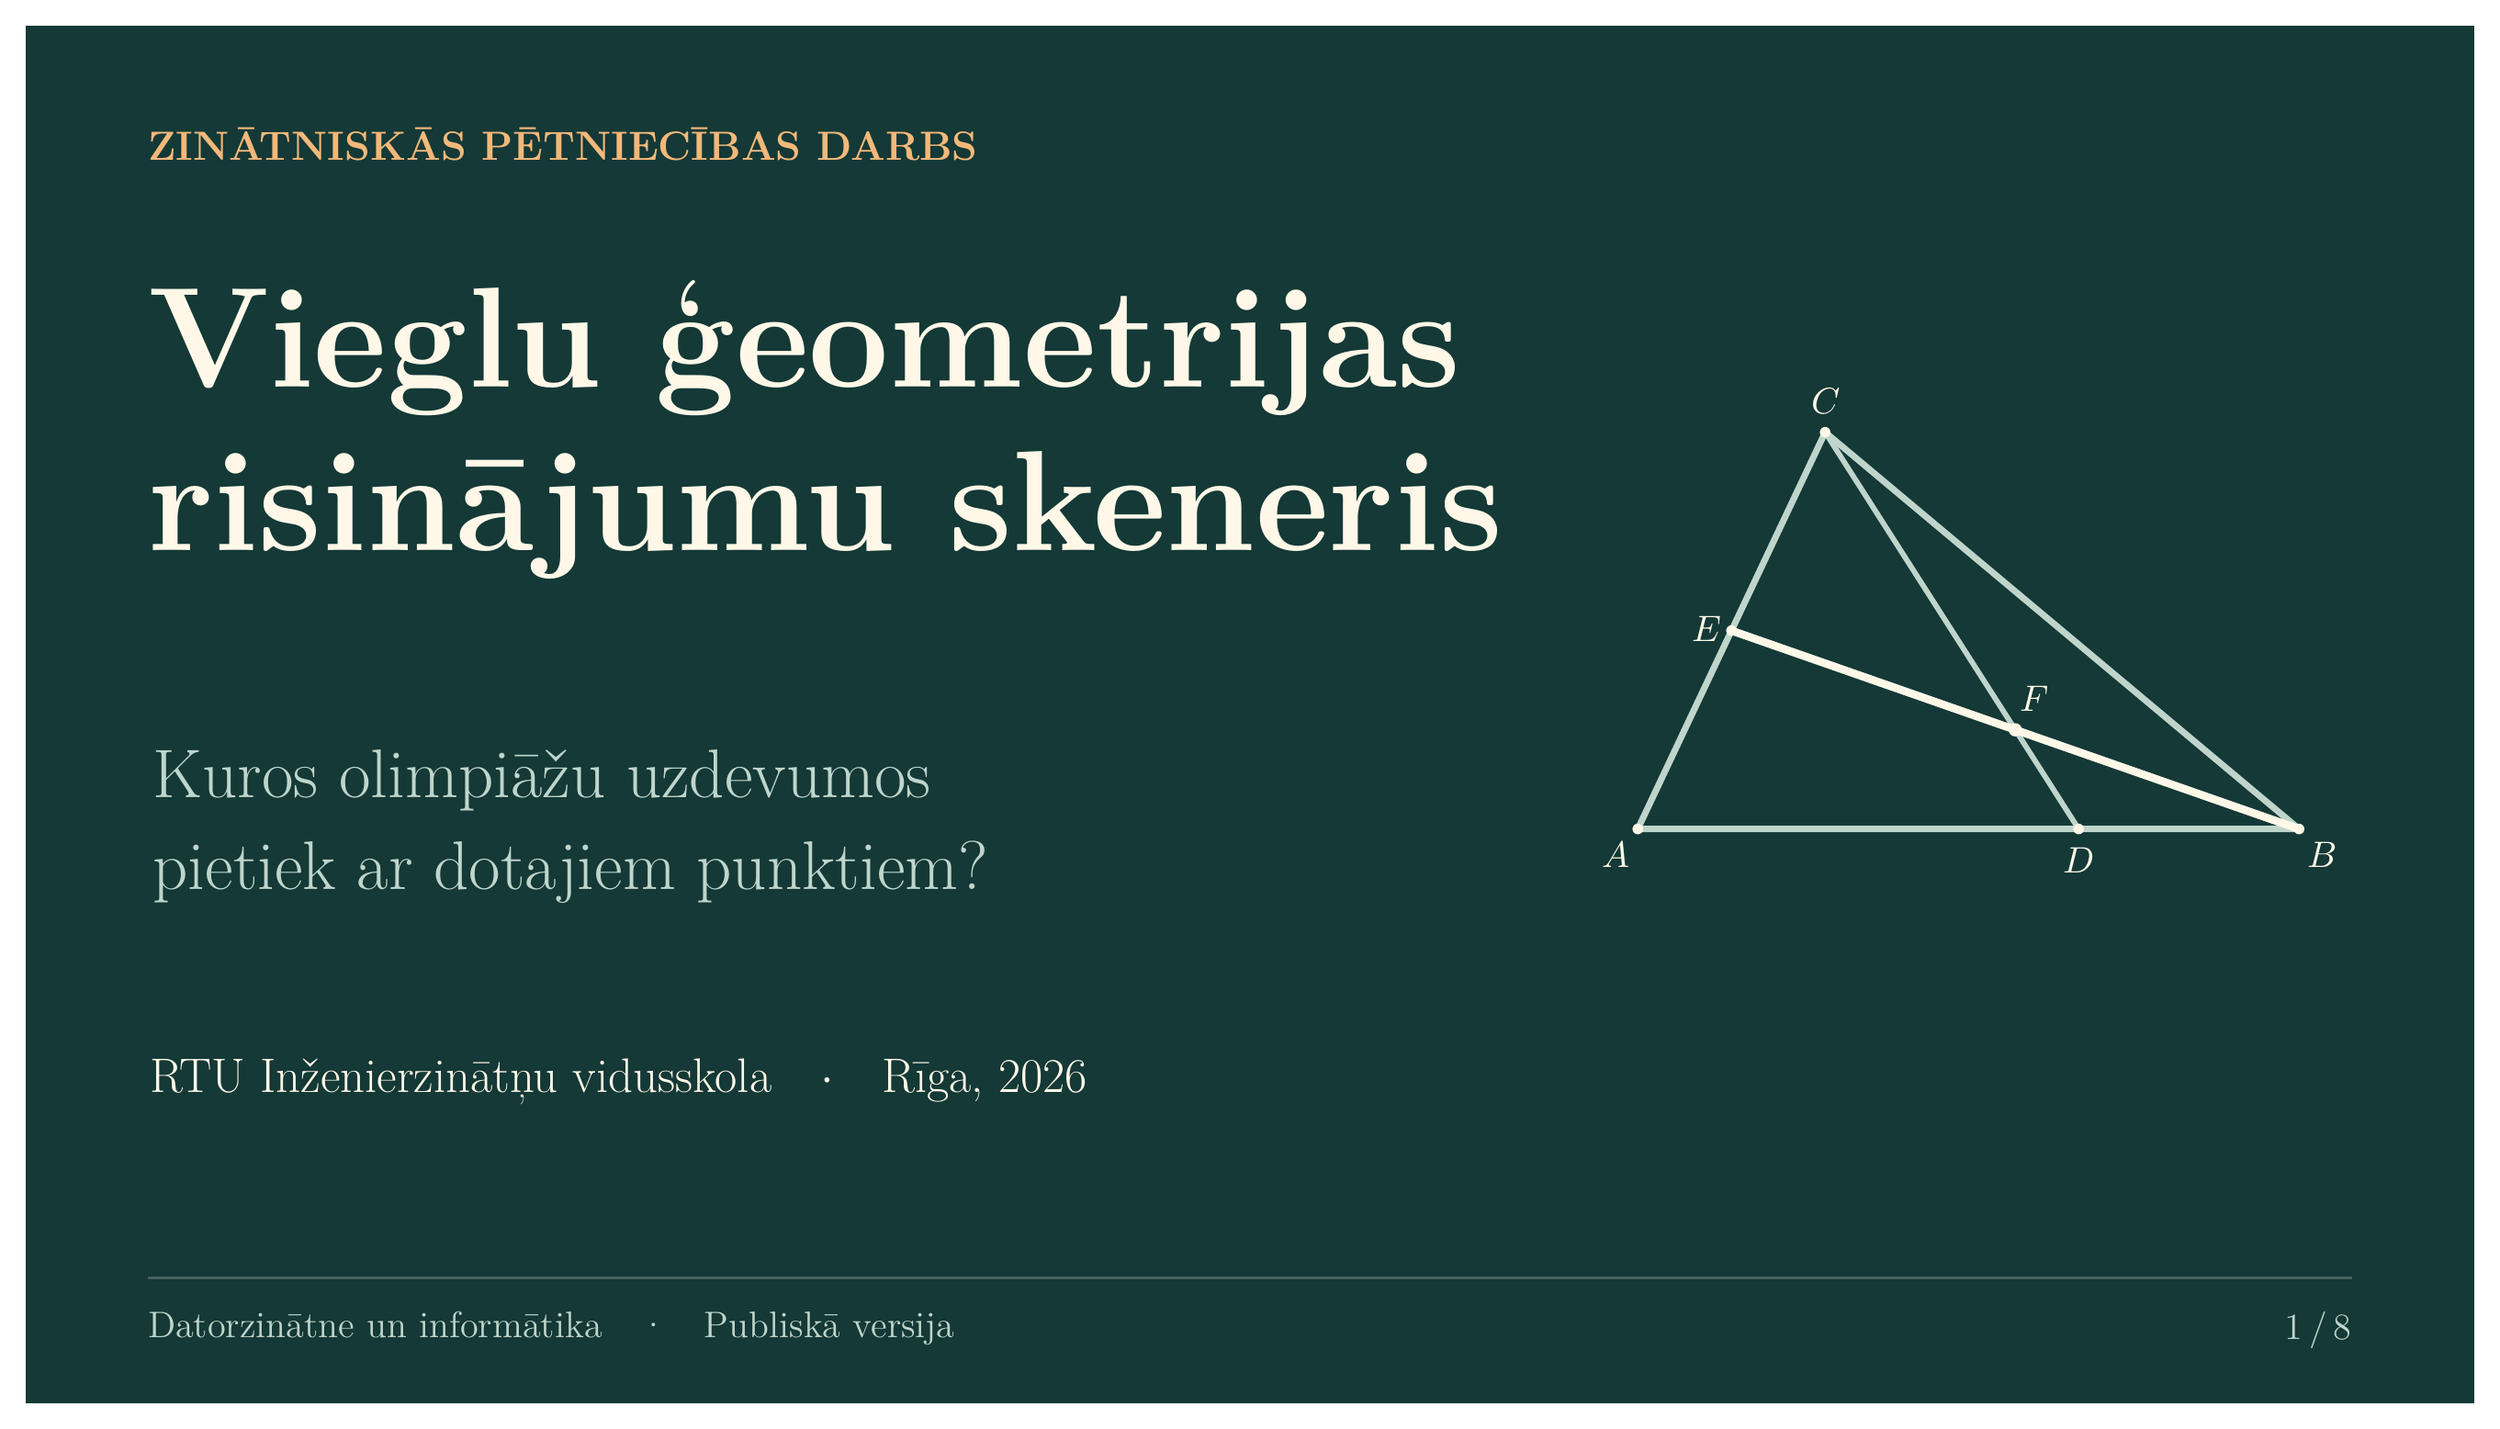
\begin{tikzpicture}[canvas]
\bg{deep}
\labelt{48}{40}{sand}{ZINĀTNISKĀS PĒTNIECĪBAS DARBS}
\type{48}{100}{580}{cream}{\sizef{56}{64}\bfseries}{Vieglu ģeometrijas\\risinājumu skeneris}
\type{50}{284}{530}{soft}{\sizef{27}{36}}{Kuros olimpiāžu uzdevumos\\pietiek ar dotajiem punktiem?}
\trianglefig{632}{315}{0.72}{1}{0}
\type{49}{405}{852}{cream}{\sizef{19}{24}}{\skola\quad $\cdot$\quad Rīga, 2026}
\ifdefempty{\autors}{}{\type{49}{439}{850}{soft}{\sizef{17}{21}}{Darba autors: \autors\ifdefempty{\vaditajs}{}{\qquad Darba vadītājs: \vaditajs}}}
\foot{dim}{soft}{Datorzinātne un informātika\quad·\quad Publiskā versija}{1}
\end{tikzpicture}
% 2. Explain what the measured outcome means.
\begin{tikzpicture}[canvas]
\bg{paper}
\labelt{48}{30}{sea}{EKSPERIMENTA UZBŪVE}
\head{ink}{Ko skeneris uzskata par risinājumu?}
\type{48}{144}{430}{sea}{\sizef{70}{77}\bfseries}{\talkCases}
\type{48}{231}{390}{ink}{\sizef{27}{34}}{formalizēti Latvijas olimpiāžu uzdevumi no \talkCandidates{} kandidātiem}
\draw[linec,line width=1bp] (468,151)--(468,382);
\type{500}{155}{407}{ink}{\sizef{27}{35}\bfseries}{Dedukcija pārbauda, ko dod zināmie fakti.}
\type{500}{255}{405}{dim}{\sizef{27}{34}}{Ja tā apstājas, meklētājs drīkst pievienot vienu jaunu palīgpunktu.}
\type{48}{419}{870}{ink}{\sizef{26}{32}}{70 ģeometrijas likumi\quad·\quad 60 sekundes mēģinājumam}
\foot{linec}{dim}{\source{\repo/blob/main/results/latvia-domain-plan.json}{Eksperimenta iestatījumi} \quad·\quad \source{\repo/tree/main/problems/latvia/geometry_translated}{Uzdevumu formalizācijas}}{2}
\end{tikzpicture}
% 3. Matched outcomes for the six completed policy configurations.
\begin{tikzpicture}[canvas]
\bg{paper}
\labelt{48}{30}{sea}{LATVIJAS UZDEVUMI}
\head{ink}{Ko mainīja algebriskā spriešana?}
\type{48}{135}{845}{dim}{\sizef{24}{30}}{Pierādītie uzdevumi no \talkCases{} katrā konfigurācijā}
\node[anchor=east,text=sea,inner sep=0] at (680,212) {\sizef{24}{28}\bfseries Ieslēgta};
\node[anchor=east,text=dim,inner sep=0] at (880,212) {\sizef{24}{28}\bfseries Izslēgta};
\foreach \y/\name/\yes/\no in {259/Dedukcija/\talkDedOn/\talkDedOff,320/Ar heiristikām/\talkHeurOn/\talkHeurOff,381/Ar modeli un heiristikām/\talkModelOn/\talkModelOff}{
    \draw[linec,line width=.8bp] (48,\y-28)--(912,\y-28);
    \node[anchor=west,inner sep=0,text=ink] at (49,\y) {\sizef{27}{32}\name};
    \node[anchor=east,inner sep=0,text=sea] at (680,\y) {\sizef{34}{38}\bfseries\yes};
    \node[anchor=east,inner sep=0,text=dim] at (880,\y) {\sizef{34}{38}\bfseries\no};
}
\type{48}{424}{864}{ink}{\sizef{23}{28}}{Tie paši \talkProvedOn{} uzdevumi visās trīs stratēģijās. Ar \talkReducedRules{} likumiem un algebrisko spriešanu dedukcija pierādīja \talkReducedWins{} no \talkCases{}.}
\foot{linec}{dim}{\source{\repo/tree/main/results/latvia-domains}{\talkRuns{} sākotnējie mēģinājumi ar pilno likumu kopu}}{3}
\end{tikzpicture}
% 4. The original geometry problem, before introducing the extra point.
\begin{tikzpicture}[canvas]
\bg{paper}
\labelt{48}{30}{sea}{LATVIJAS 75. MATEMĀTIKAS OLIMPIĀDE · 9. KLASE}
\head{ink}{Kāpēc $F$ ir mediānas viduspunkts?}
\trianglefig{72}{407}{1.12}{0}{0}
\type{535}{169}{372}{ink}{\sizef{29}{38}}{$AD:DB=2:1$.\\ $E$ ir $AC$ viduspunkts.}
\type{535}{280}{360}{dim}{\sizef{26}{34}}{$BE$ un $CD$ krustojas\\punktā $F$.}
\type{535}{385}{370}{sea}{\sizef{30}{38}\bfseries}{Jāpierāda \mbox{$BF=FE$.}}
\foot{linec}{dim}{\source{\nmsproblem}{LU NMS · 2024./25. gada valsts olimpiādes 9.2. uzdevums}}{4}
\end{tikzpicture}
% 5. Geometric inference; the additional point was present in the formalization.
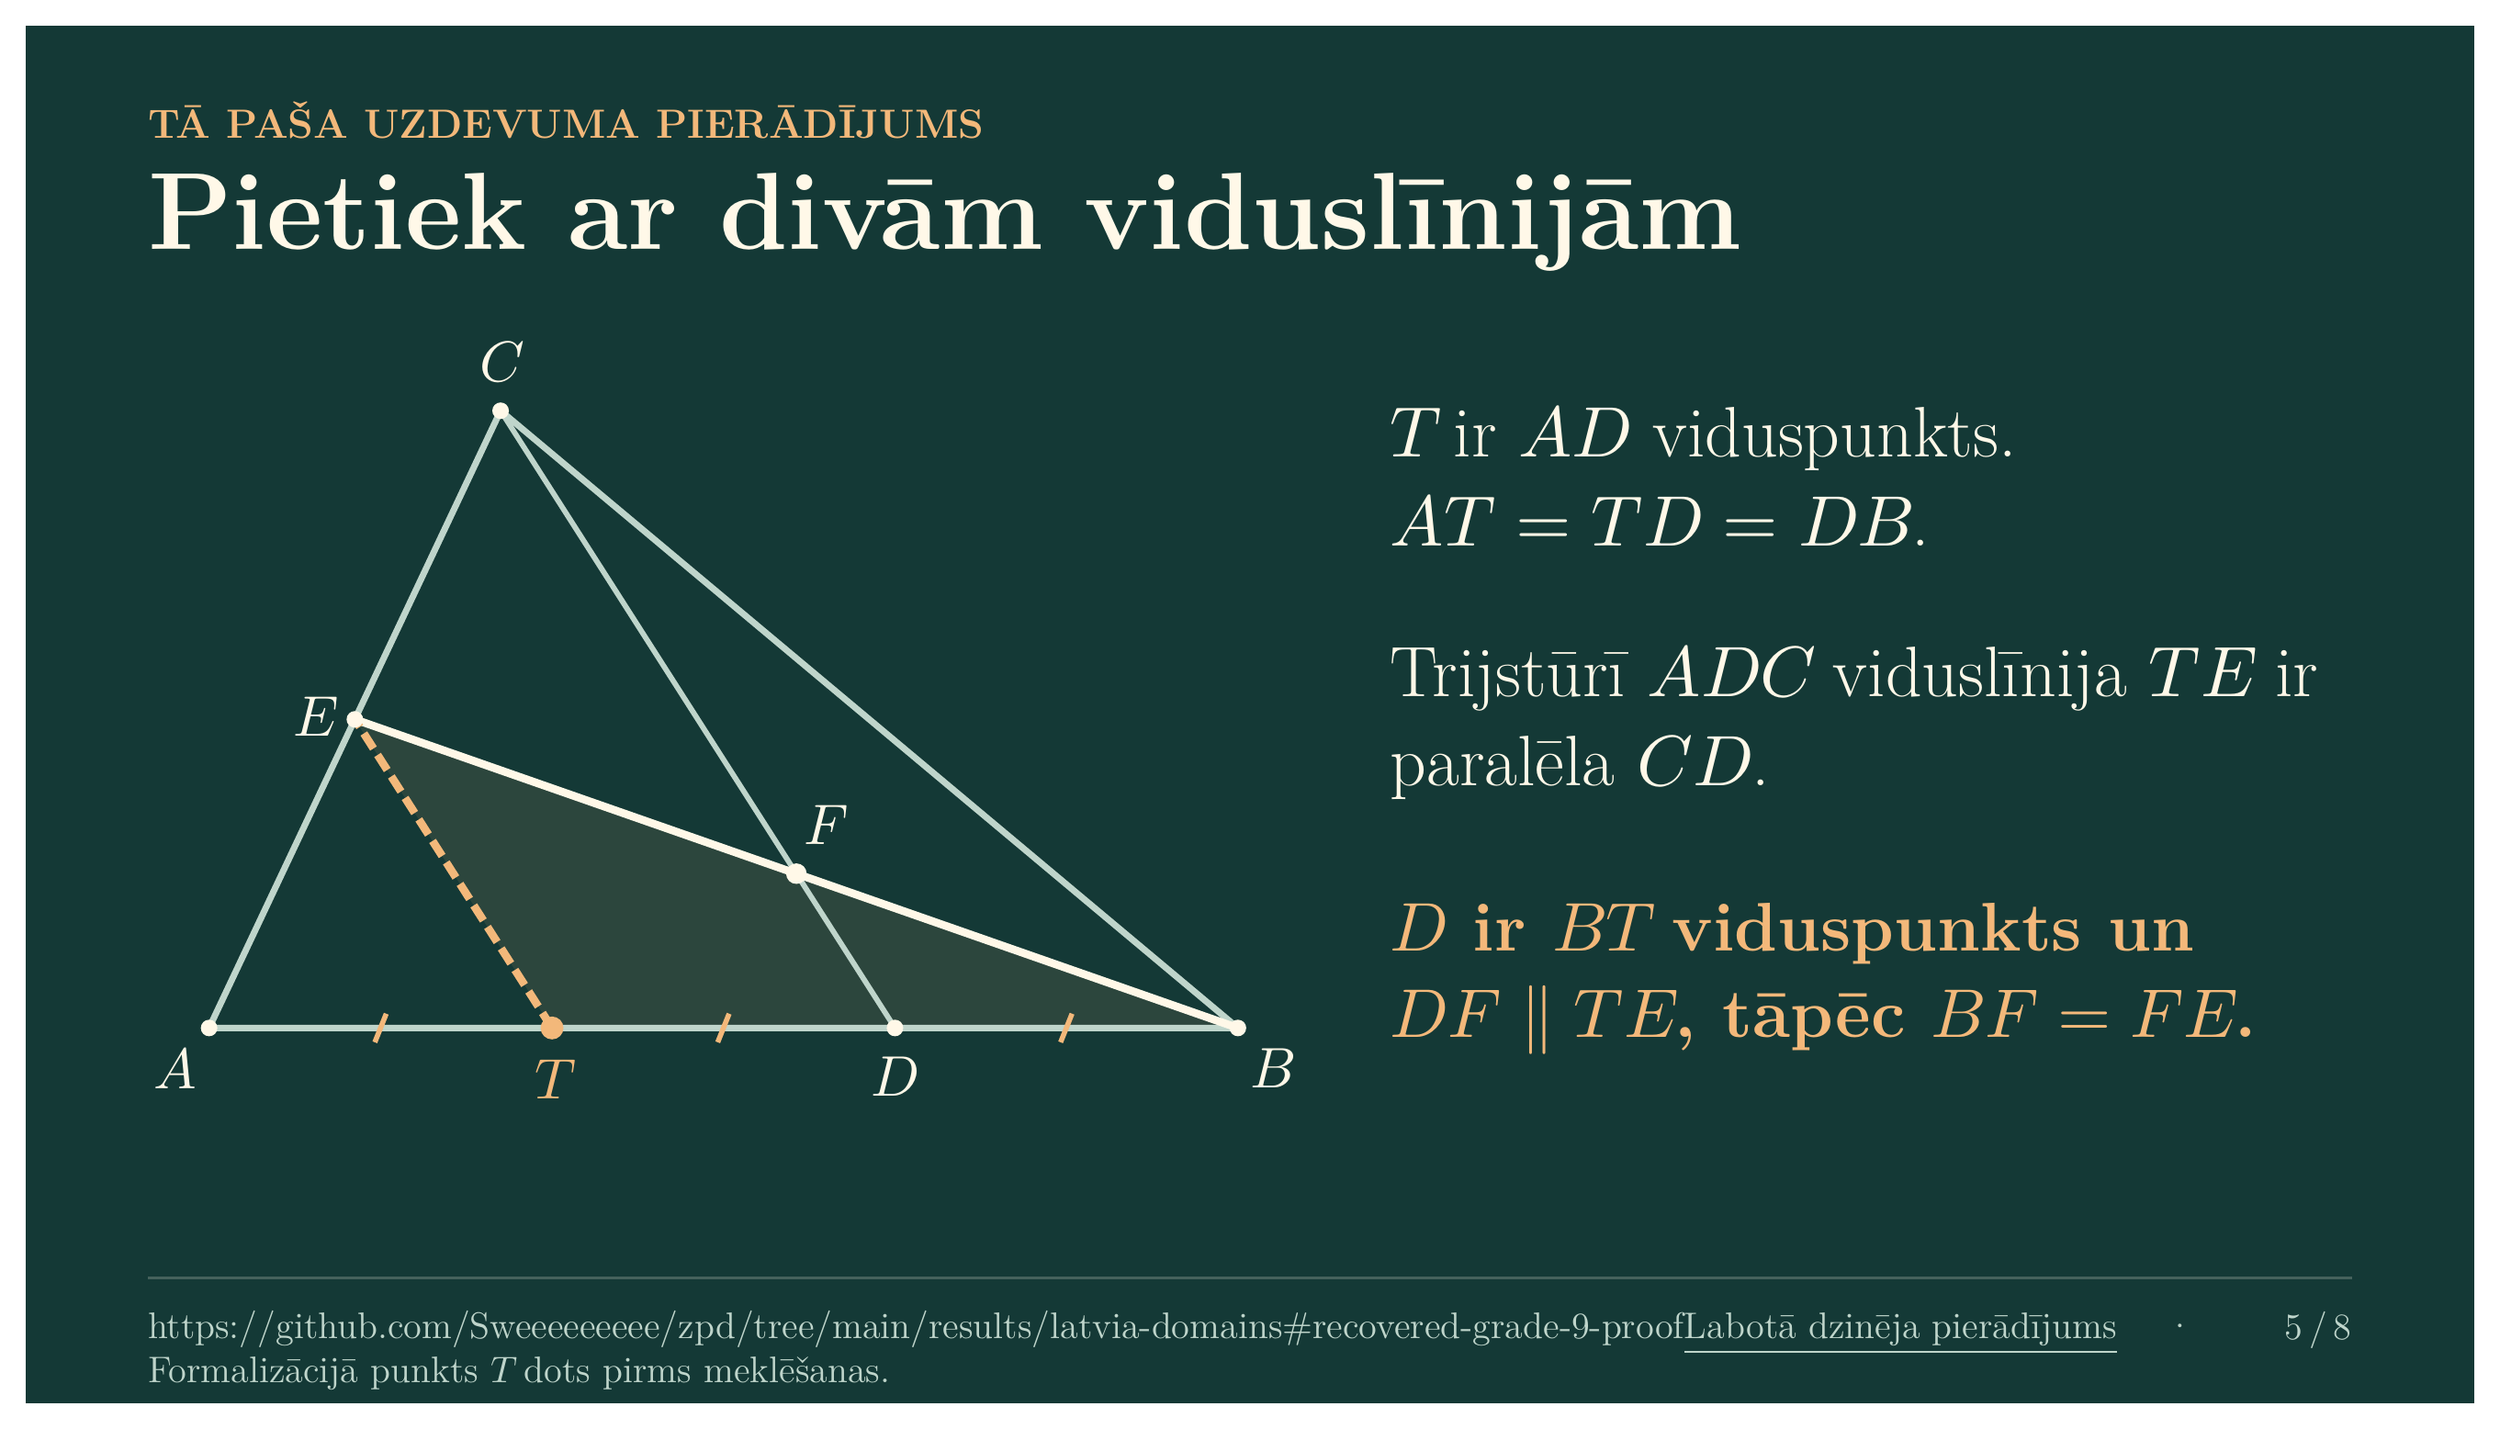
\begin{tikzpicture}[canvas]
\bg{deep}
\labelt{48}{30}{sand}{TĀ PAŠA UZDEVUMA PIERĀDĪJUMS}
\head{cream}{Pietiek ar divām viduslīnijām}
\trianglefig{72}{393}{1.12}{1}{1}
\type{535}{149}{385}{cream}{\sizef{28}{35}}{$T$ ir $AD$ viduspunkts.\\ $AT=TD=DB$.}
\type{535}{243}{383}{cream}{\sizef{28}{35}}{Trijstūrī $ADC$ viduslīnija $TE$ ir paralēla $CD$.}
\type{535}{344}{380}{sand}{\sizef{27}{34}\bfseries}{$D$ ir $BT$ viduspunkts un \mbox{$DF\parallel TE$,} tāpēc \mbox{$BF=FE$.}}
\foot{dim}{soft}{\source{\repo/tree/main/results/latvia-domains\#recovered-grade-9-proof}{Labotā dzinēja pierādījums} \quad·\quad Formalizācijā punkts $T$ dots pirms meklēšanas.}{5}
\end{tikzpicture}
% 6. Separate prediction and theorem-proving denominators.
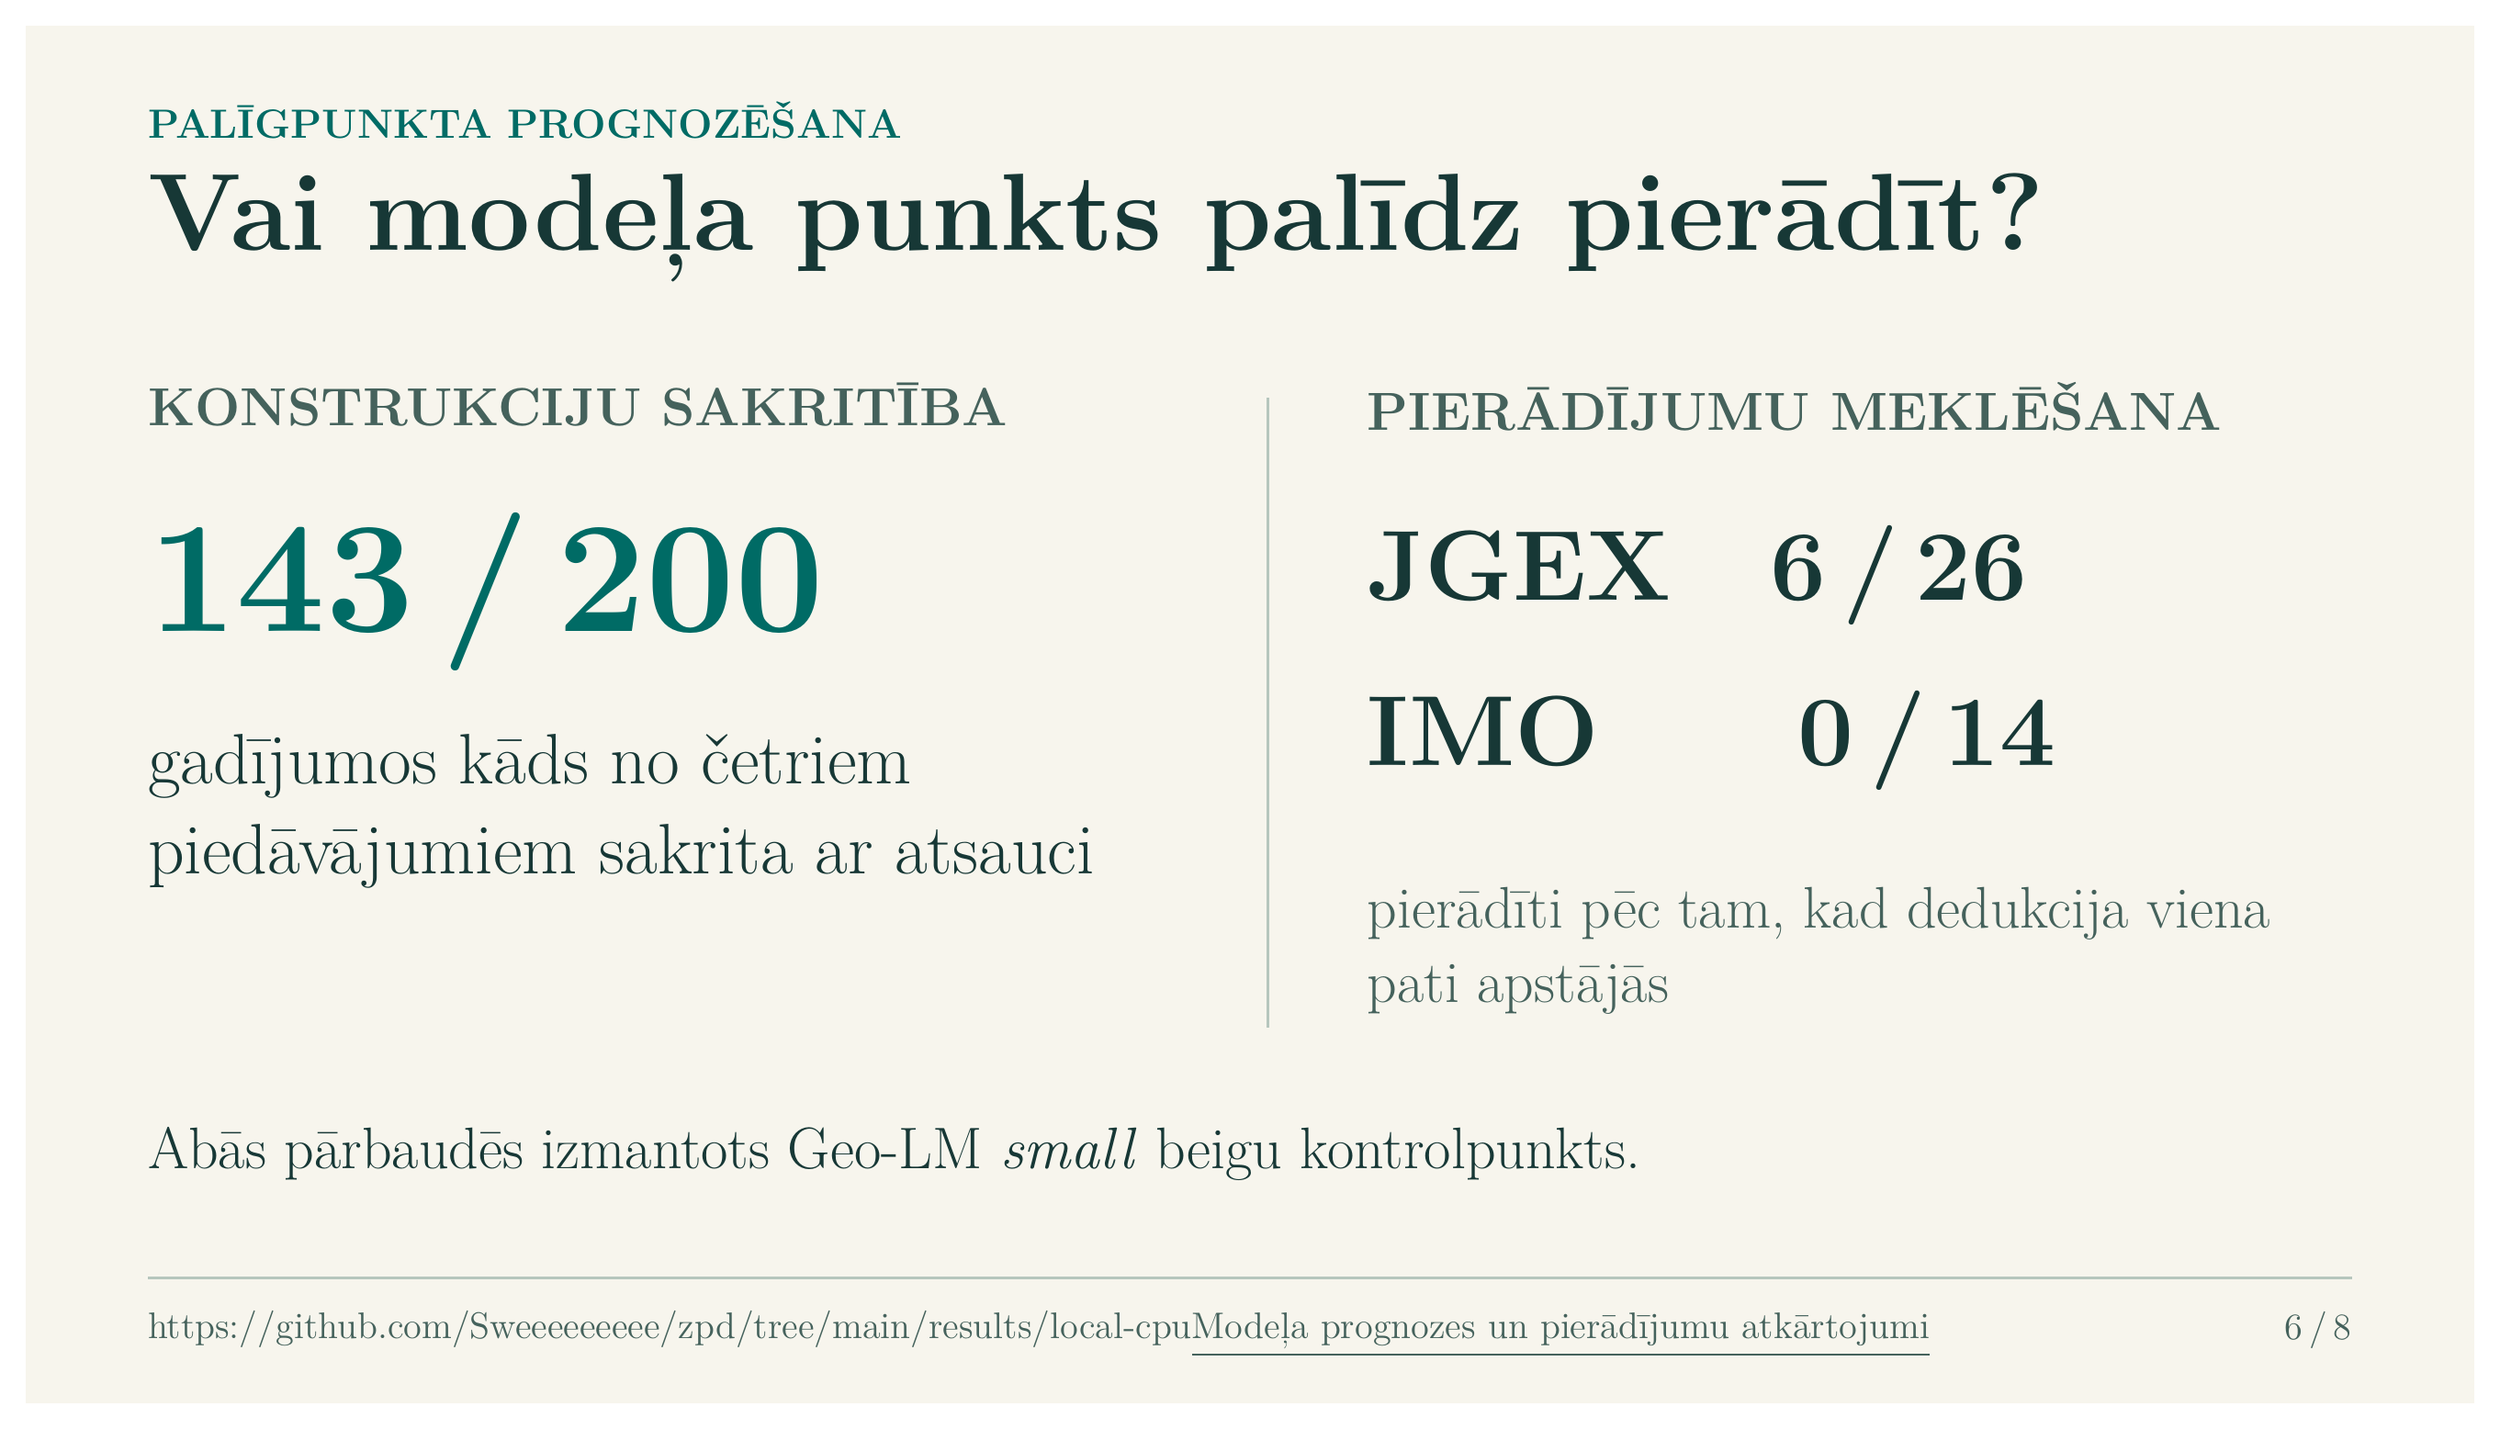
\begin{tikzpicture}[canvas]
\bg{paper}
\labelt{48}{30}{sea}{PALĪGPUNKTA PROGNOZĒŠANA}
\head{ink}{Vai modeļa punkts palīdz pierādīt?}
\type{48}{140}{420}{dim}{\sizef{21}{26}\bfseries}{KONSTRUKCIJU SAKRITĪBA}
\type{48}{191}{405}{sea}{\sizef{62}{67}\bfseries}{\talkTopFour\,/\,\talkPredCases}
\type{48}{278}{395}{ink}{\sizef{28}{35}}{gadījumos kāds no četriem piedāvājumiem sakrita ar atsauci}
\draw[linec,line width=1bp] (487,146)--(487,393);
\type{526}{140}{382}{dim}{\sizef{21}{26}\bfseries}{PIERĀDĪJUMU MEKLĒŠANA}
\type{526}{196}{370}{ink}{\sizef{39}{47}\bfseries}{JGEX\quad \talkJgexWon\,/\,\talkJgexTried}
\type{526}{261}{370}{ink}{\sizef{39}{47}\bfseries}{IMO\qquad \talkImoWon\,/\,\talkImoTried}
\type{526}{338}{370}{dim}{\sizef{23}{29}}{pierādīti pēc tam, kad dedukcija viena pati apstājās}
\type{48}{432}{861}{ink}{\sizef{23}{29}}{Abās pārbaudēs izmantots Geo-LM \textit{small} beigu kontrolpunkts.}
\foot{linec}{dim}{\source{\repo/tree/main/results/local-cpu}{Modeļa prognozes un pierādījumu atkārtojumi}}{6}
\end{tikzpicture}
% 7. Audit of the printed algebraic steps.
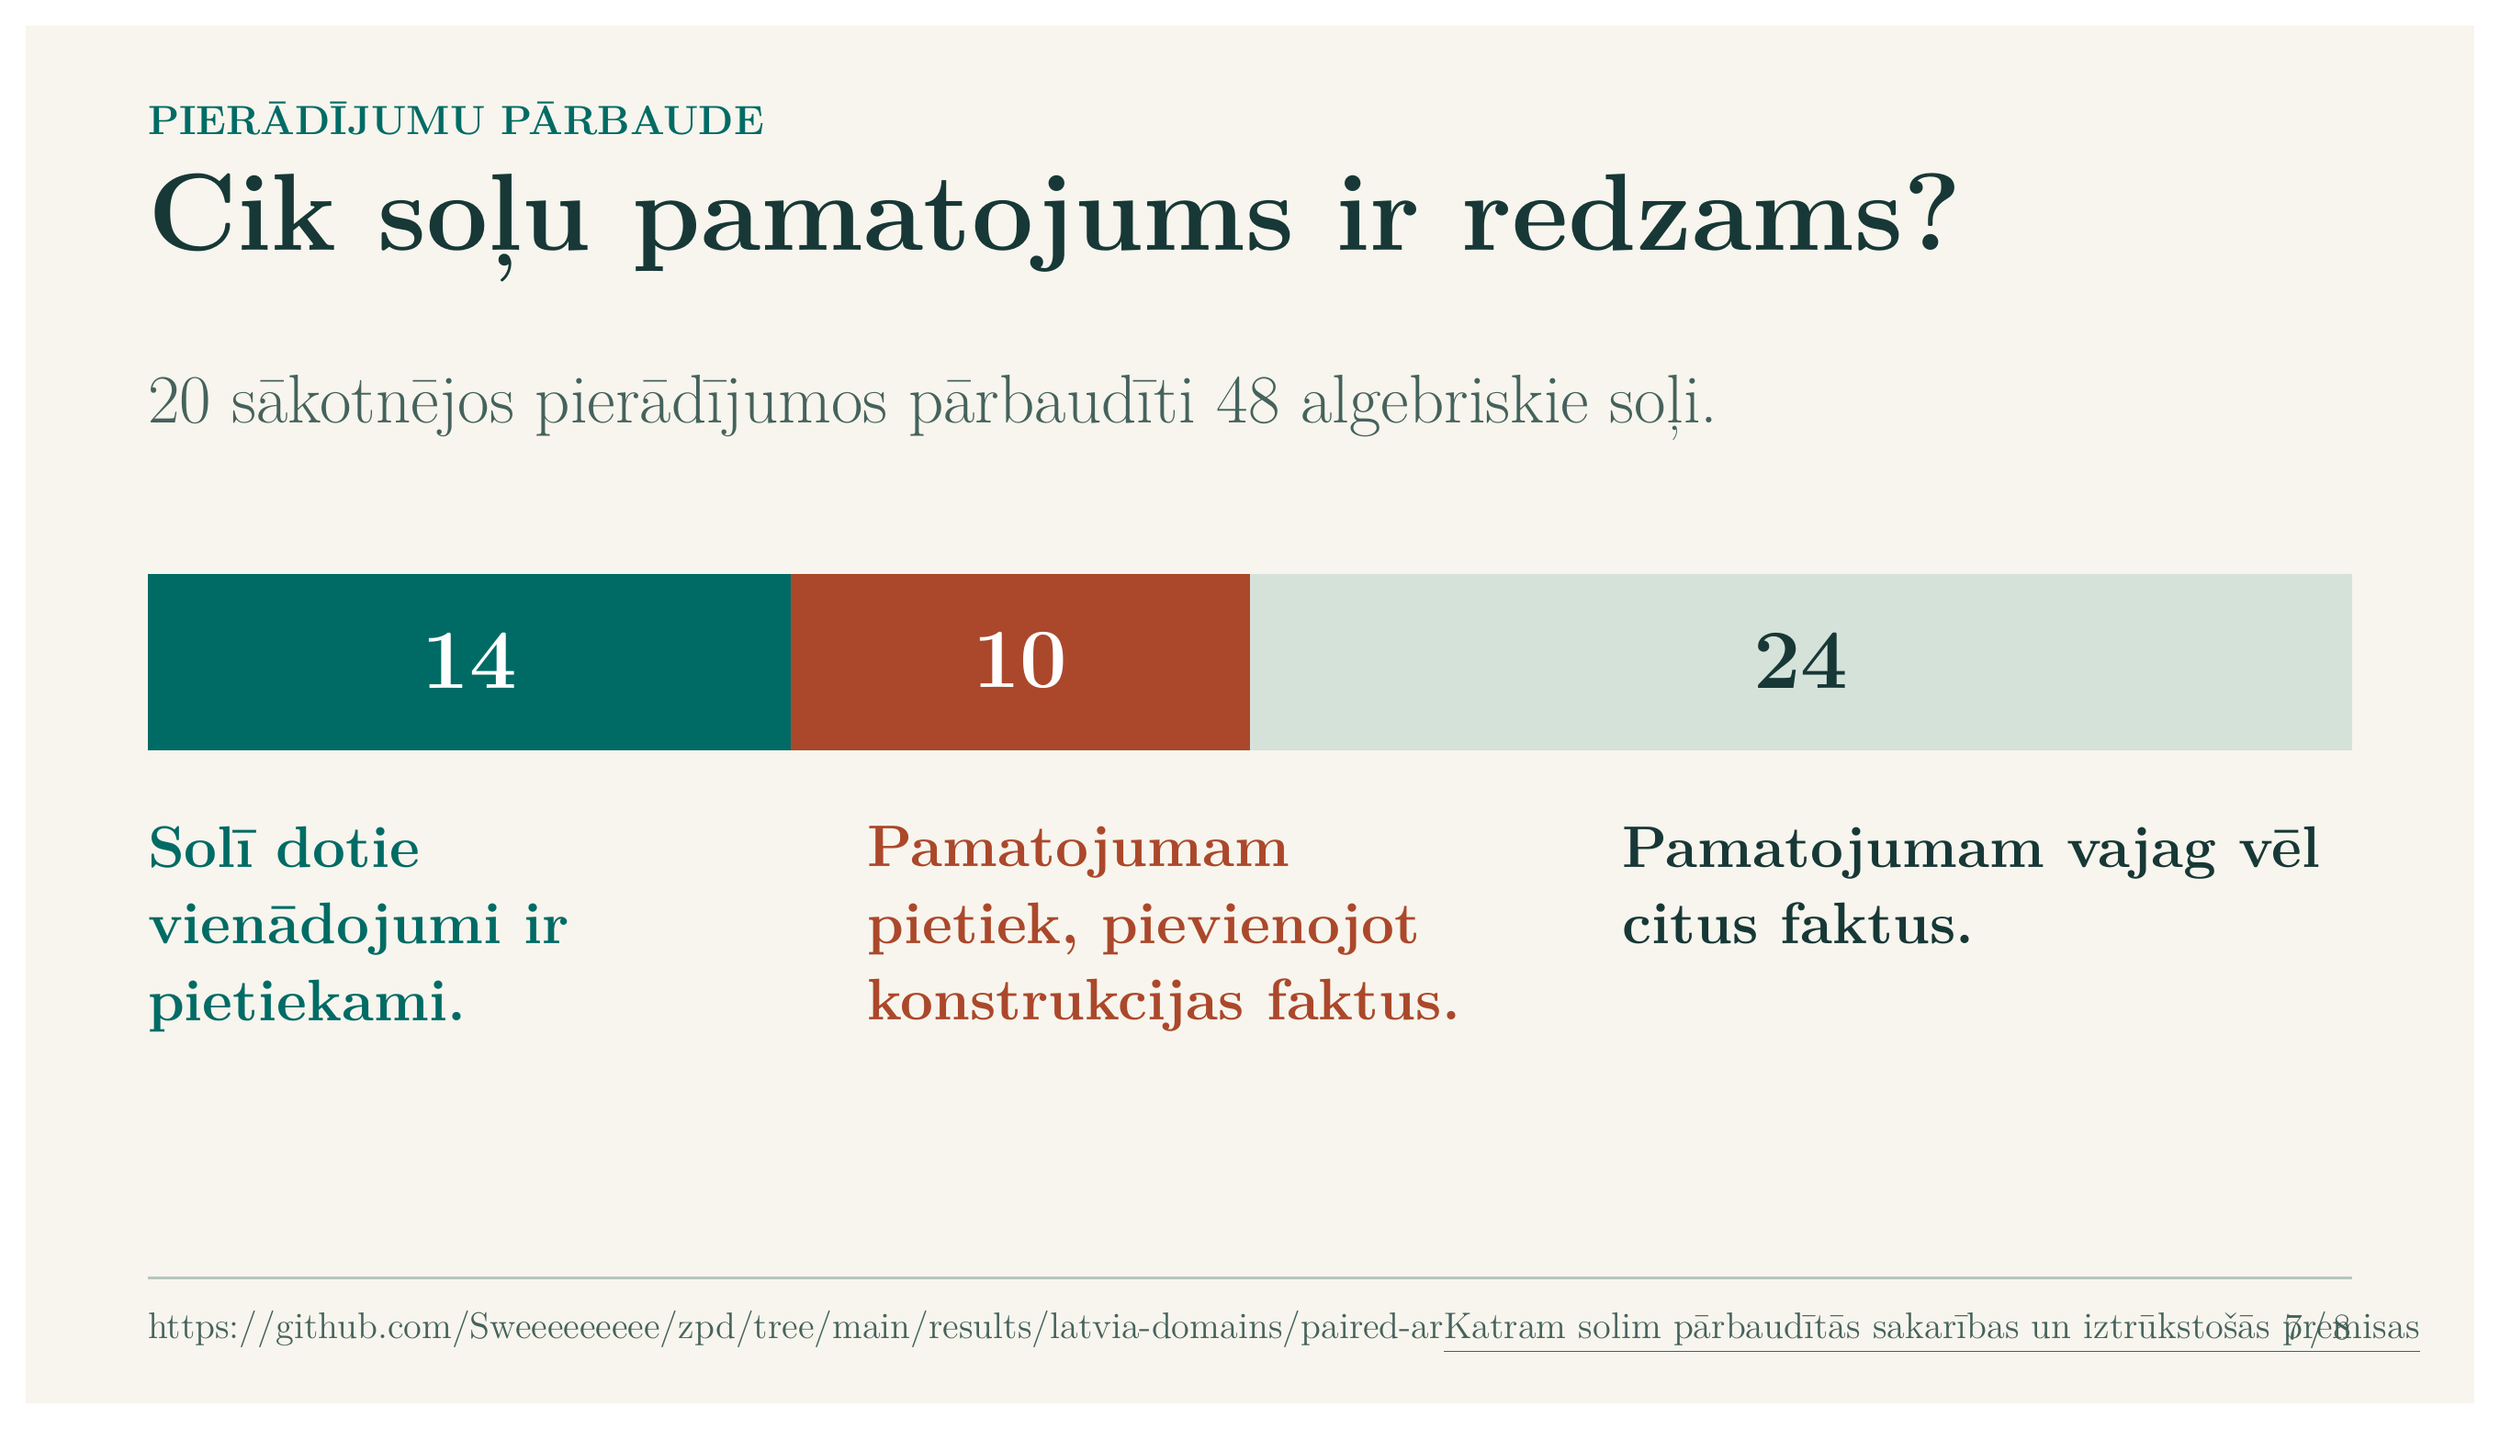
\begin{tikzpicture}[canvas]
\bg{paper}
\labelt{48}{30}{sea}{PIERĀDĪJUMU PĀRBAUDE}
\head{ink}{Cik soļu pamatojums ir redzams?}
\type{48}{137}{860}{dim}{\sizef{27}{34}}{\talkTranscripts{} sākotnējos pierādījumos pārbaudīti \talkSteps{} algebriskie soļi.}
\pgfmathsetmacro{\cutA}{48+(864/\talkSteps)*\talkExplicit}
\pgfmathsetmacro{\cutB}{48+(864/\talkSteps)*(\talkExplicit+\talkReconstructed)}
\fill[sea] (48,215) rectangle (\cutA,284);
\fill[clay] (\cutA,215) rectangle (\cutB,284);
\fill[pale] (\cutB,215) rectangle (912,284);
\node[text=white] at ({(48+\cutA)/2},249) {\sizef{33}{38}\bfseries\talkExplicit};
\node[text=white] at ({(\cutA+\cutB)/2},249) {\sizef{33}{38}\bfseries\talkReconstructed};
\node[text=ink] at ({(\cutB+912)/2},249) {\sizef{33}{38}\bfseries\talkUnresolved};
\type{48}{314}{251}{sea}{\sizef{23}{30}\bfseries}{Solī dotie vienādojumi ir pietiekami.}
\type{330}{314}{255}{clay}{\sizef{23}{30}\bfseries}{Pamatojumam pietiek, pievienojot konstrukcijas faktus.}
\type{626}{314}{285}{ink}{\sizef{23}{30}\bfseries}{Pamatojumam vajag vēl citus faktus.}
\foot{linec}{dim}{\source{\repo/tree/main/results/latvia-domains/paired-ar}{Katram solim pārbaudītās sakarības un iztrūkstošās premisas}}{7}
\end{tikzpicture}
% 8. Human scores and the limits of the conclusion.
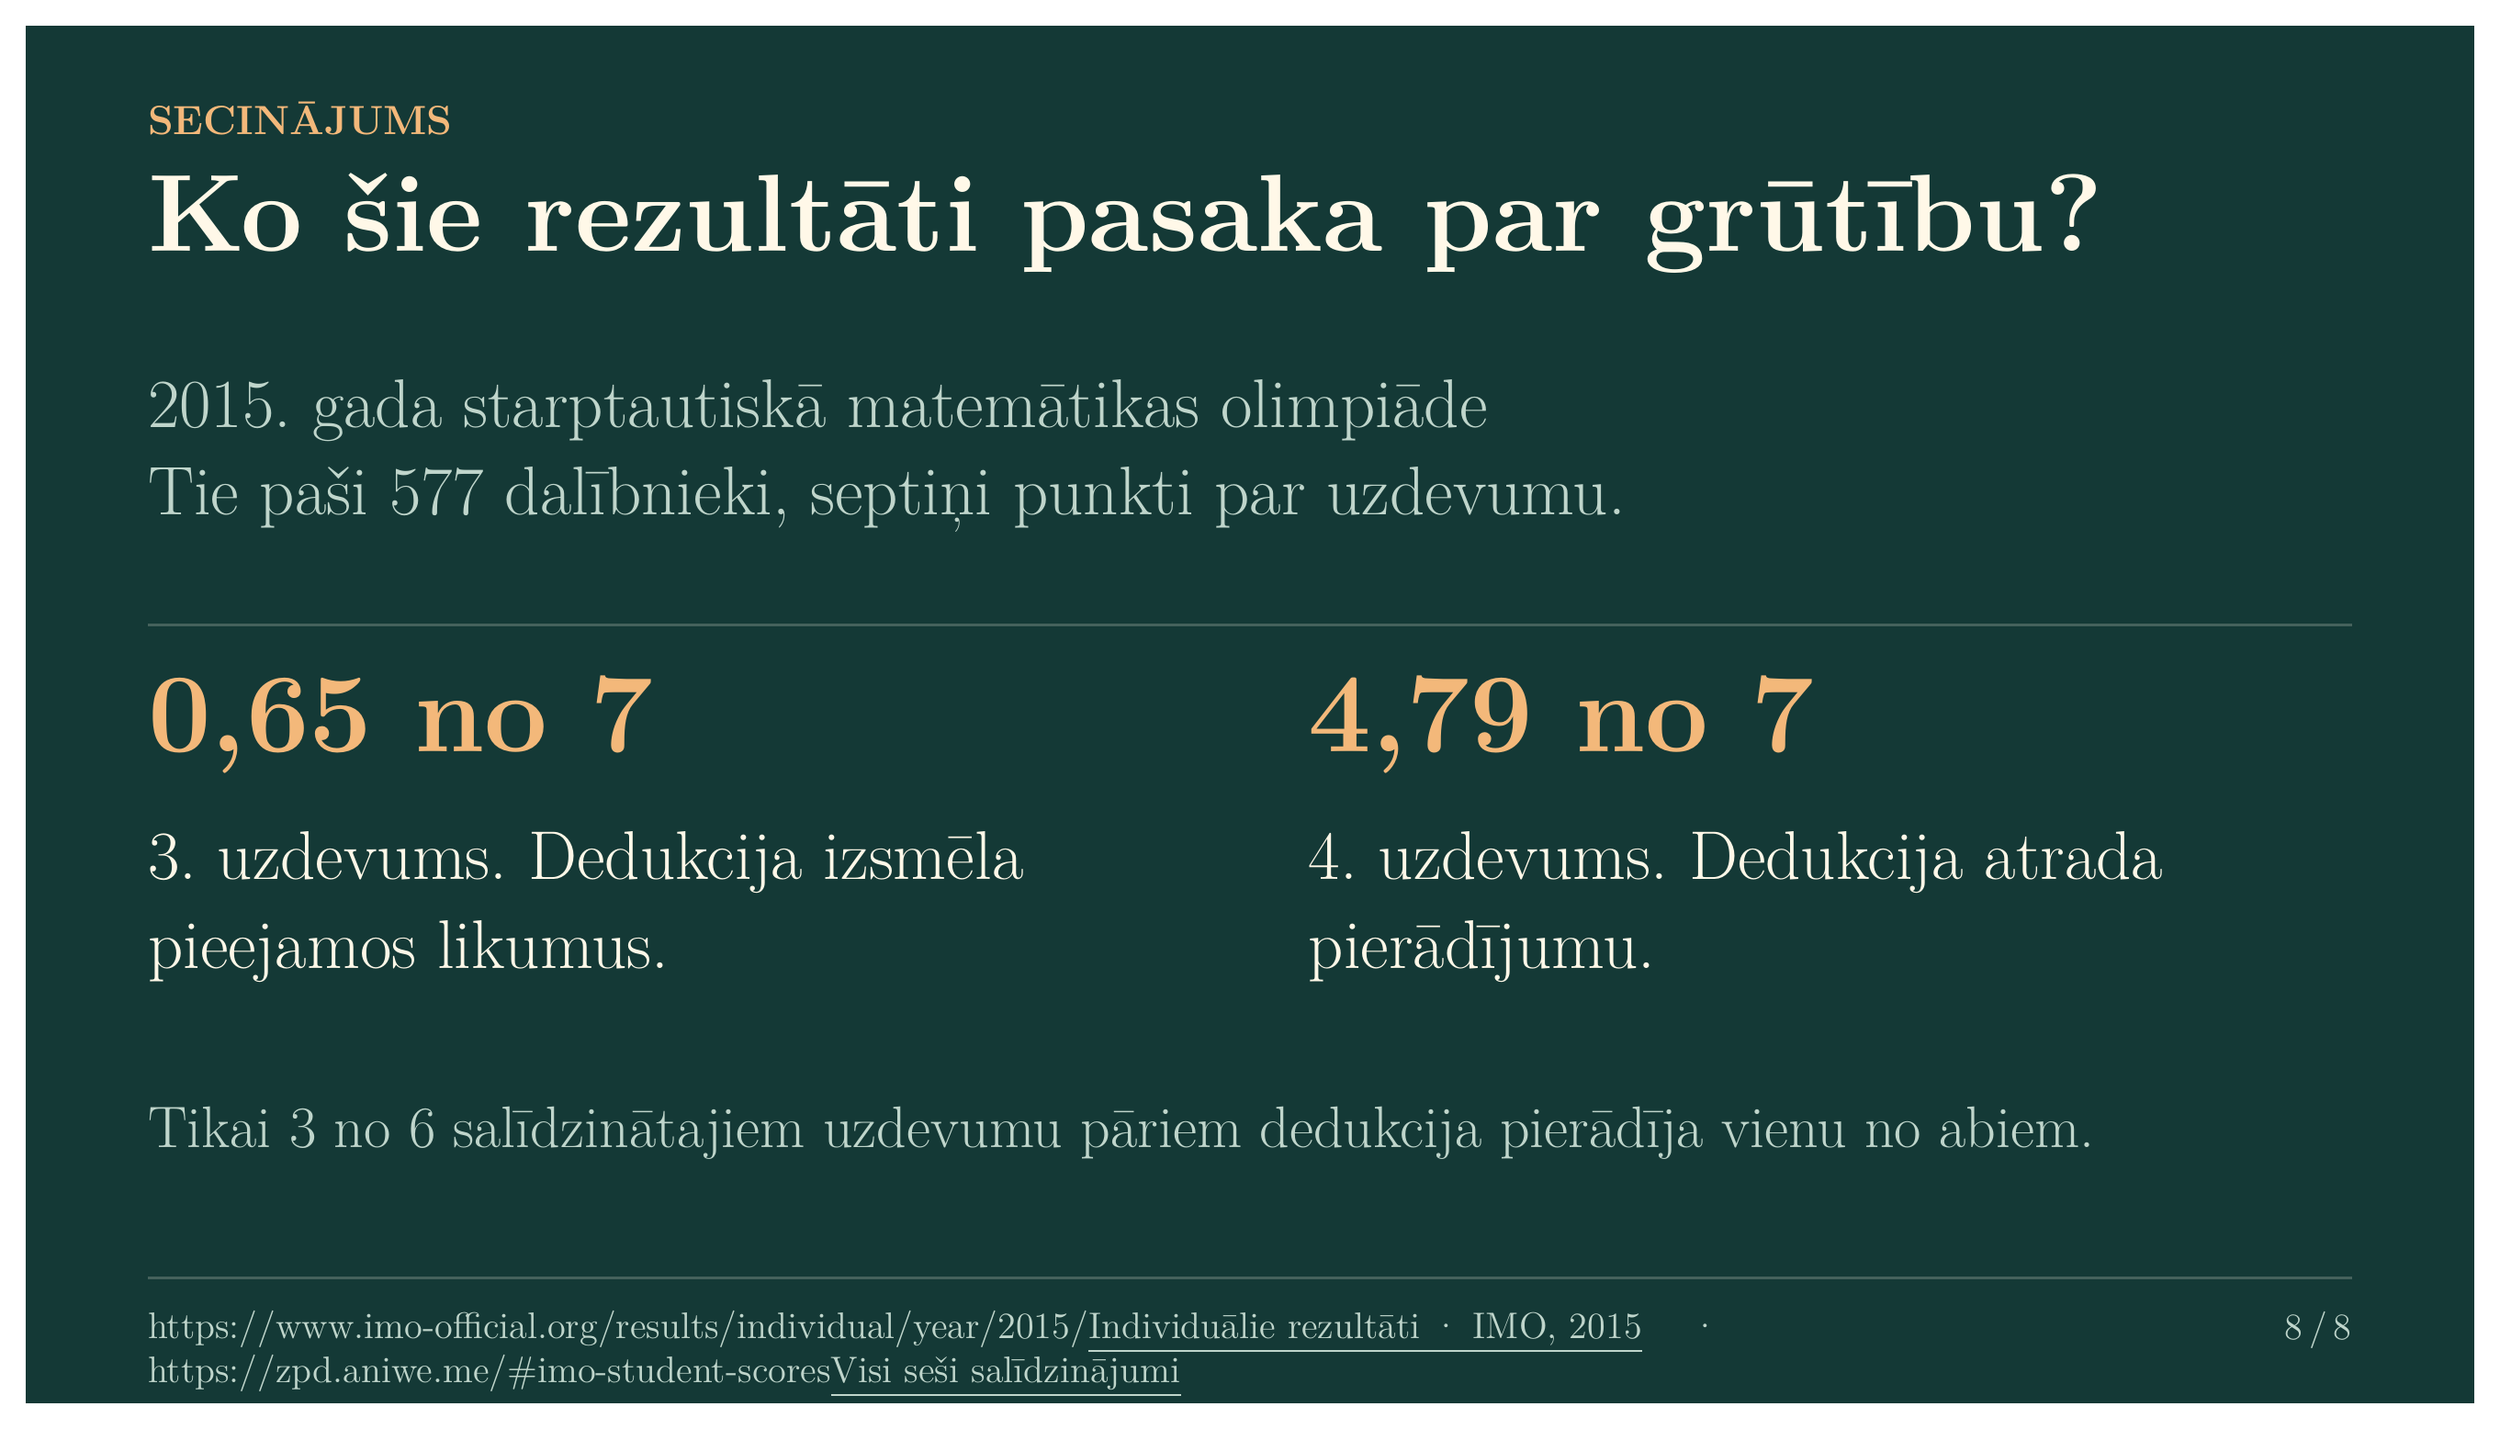
\begin{tikzpicture}[canvas]
\bg{deep}
\labelt{48}{30}{sand}{SECINĀJUMS}
\head{cream}{Ko šie rezultāti pasaka par grūtību?}
\type{48}{139}{860}{soft}{\sizef{27}{34}}{2015. gada starptautiskā matemātikas olimpiāde\\Tie paši \talkImoParticipants{} dalībnieki, septiņi punkti par uzdevumu.}
\draw[dim,line width=1bp] (48,235)--(912,235);
\type{48}{255}{420}{sand}{\sizef{44}{50}\bfseries}{\talkImoThreeMean{} no 7}
\type{48}{316}{413}{cream}{\sizef{27}{35}}{3. uzdevums. Dedukcija izsmēla pieejamos likumus.}
\type{503}{255}{407}{sand}{\sizef{44}{50}\bfseries}{\talkImoFourMean{} no 7}
\type{503}{316}{405}{cream}{\sizef{27}{35}}{4. uzdevums. Dedukcija atrada pierādījumu.}
\type{48}{424}{871}{soft}{\sizef{23}{29}}{Tikai \talkHigher{} no \talkCohorts{} salīdzinātajiem uzdevumu pāriem dedukcija pierādīja vienu no abiem.}
\foot{dim}{soft}{\source{\imoscores}{Individuālie rezultāti · IMO, 2015} \quad·\quad \source{https://zpd.aniwe.me/\#imo-student-scores}{Visi seši salīdzinājumi}}{8}
\end{tikzpicture}
\end{document}
